\section{Notation}%
\label{sec:notation}
\begin{figure}
  \begin{subfigure}{.5\textwidth}
    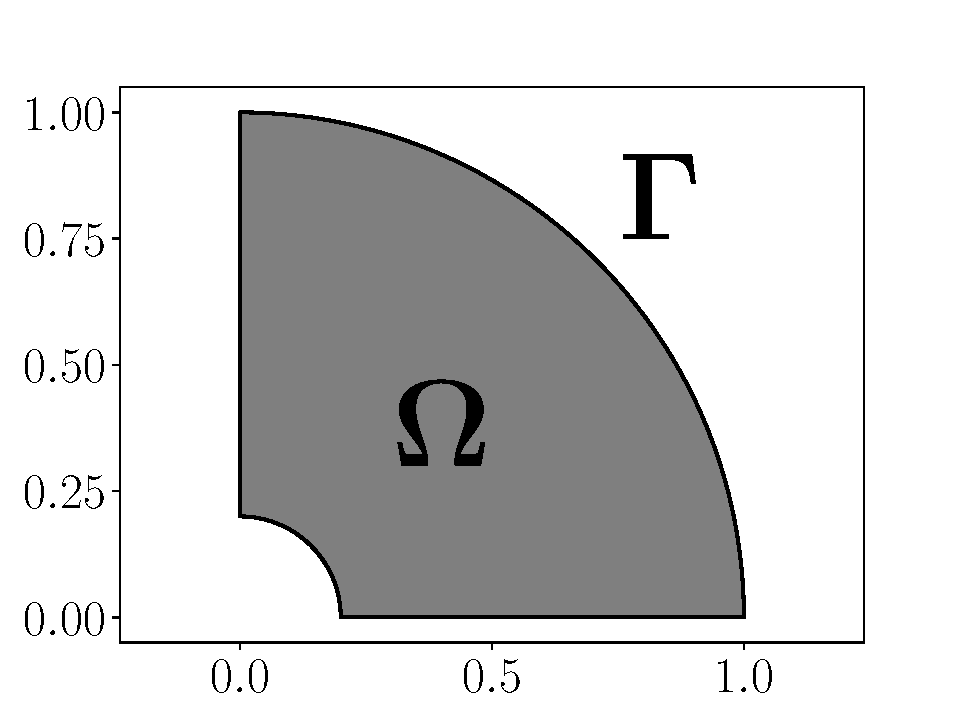
\includegraphics[width=\textwidth]{images/domain.pdf}%
    \caption{An annulus sector domain.}%
    \label{fig:domain}
  \end{subfigure}
  \begin{subfigure}{.5\textwidth}
    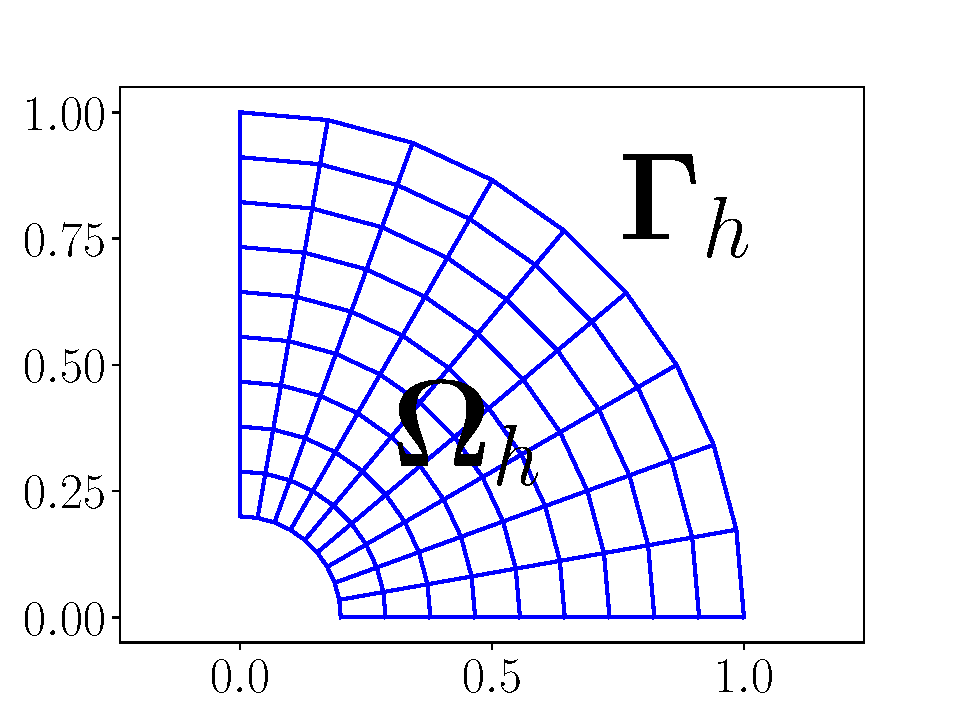
\includegraphics[width=\textwidth]{images/grid.pdf}%
    \caption{A discretization of $\Omega$.}%
    \label{fig:grid}
  \end{subfigure}
  \caption{A curved domain $\Omega$ and a named boundary $\Gamma$.}
\end{figure}
In the continuous setting we consider time dependent scalar- and vector-valued functions on a spatial domain $\Omega$ (such as in Figure~\ref{fig:domain}). Vector-valued functions are column vectors and indicated with an arrow, for example
$
  \vec{w} =
  \begin{pmatrix}
    u & v
  \end{pmatrix}^\top
$
denoting the velocity field. Let $\phic, \psic : \Omega \to \mathbb{R}^n$. We denote by $\normc{\phic}$ and $\ipc{\phic}{\psic}$ the $L^2$ inner product and norm on $\Omega$ respectively,
\begin{equation*}
  \ipc{\phic}{\psic} := \int_\Omega \phic \cdot \psic dx dy \,, \quad \normc{\phic} := \sqrt{\int_\Omega |\phic|^2 dxdy} \,.
\end{equation*}
Similarly, the $L^2$ inner product on $\partial \Omega$ is denoted $\ipbc{\cdot}{\cdot}$,
\begin{equation*}
  \ipbc{\phic}{\psic} := \int_{\partial \Omega} \phic \cdot \psic ds \,.
\end{equation*}
Recall the definitions of the gradient ($\nabla$) and divergence ($\div$) operators,
\begin{equation*}
  \nabla u = (u_x, u_y), \quad \div\wc = u_x + v_y \,,
\end{equation*}
and Green's identity,
\begin{equation}
  \label{eq:greens_identity}
  \ipc{\phic}{\nabla\psi} = \ipbc{\phic \cdot \nc}{\psi} - \ipc{\div \phic}{\psi} \,.
\end{equation}
where $\nc$ is the outward point unit normal of the boundary $\partial \Omega$. We allow the gradient, the divergence, and the dot product to operate row-wise, so that for example
\begin{equation*}
  \wc \cdot \nabla \wc =
  \begin{pmatrix}
    \wc \cdot \nabla u \\
    \wc \cdot \nabla v
  \end{pmatrix}
  =
  \begin{pmatrix}
    u u_x + v u_y \\
    u v_x + v v_y
  \end{pmatrix}
\end{equation*}
and
\begin{equation*}
  \div \wc \wc^\top =
  \div
  \begin{pmatrix}
    uu & uv \\
    uv & vv
  \end{pmatrix}
  =
  \begin{pmatrix}
    {(uu)}_x + {(uv)}_y \\
    {(uv)}_x + {(vv)}_y
  \end{pmatrix} \,.
\end{equation*}

The semi-discrete setting mimics the continuous setting to a large extent, with a few caveats (such as no product rule for differentiation). Notationally we will see that the continuous and discrete settings are virtually identical.

Consider an $N_x$-by-$N_y$ curvilinear grid $\Omega_h$ as in Figure~\ref{fig:grid}. We think of our semi-discrete solutions as column vectors of function evaluations on this grid, denoted in bold. For example, if
$
  u : \Omega \to \mathbb{R}
$,
then
$
  \un =
  \begin{pmatrix}
    \un_1^\top & \un_2^\top & \cdots & \un_{N_x}^\top
  \end{pmatrix}^\top
$,
where
\[
  \un_i =
  \begin{pmatrix}
    u_{i1} & u_{i2} & \cdots & u_{iN_y}
  \end{pmatrix}^\top
  \approx
  \begin{pmatrix}
    u(x_{i1}, y_{i1}) & u(x_{i2}, y_{i2}) & \cdots & u(x_{iN_y}, y_{iN_y})
  \end{pmatrix}^\top \,.
\]

Note that $\un$ is a special kind of vector in that its purpose is to approximate a continuous function. To make this distinction clear let us make a formal definition.

\begin{definition}
  Given an $N_x$-by-$N_y$ curvilinear grid $\Omega_h$, a vector $\un \in \mathbb{R}^{N_x N_y}$ is called a \emph{grid function}.
\end{definition}

We make extensive use of elementwise operations on grid functions. If $\un$ and $\vn$ are grid functions, then the elementwise product is indicated with no symbol,
\begin{equation*}
  \un\vn =
  \begin{pmatrix}
    u_{11}v_{11} & u_{12}v_{12} & \cdots & u_{21}v_{21} & u_{22}v_{22} & \cdots
  \end{pmatrix}^\top \,.
\end{equation*}
Similarly elementwise fractions are indicated by a division symbol,
\begin{equation*}
  \un/\vn =
  \begin{pmatrix}
    u_{11}/v_{11} & u_{12}/v_{12} & \cdots & u_{21}/v_{21} & u_{22}/v_{22} & \cdots
  \end{pmatrix}^\top \,.
\end{equation*}
For a scalar function $h : \mathbb{R} \to \mathbb{R}$ we will write $h(\un)$ to indicate elementwise application of $h$ to $\un$,
\begin{equation*}
  h(\un) =
  \begin{pmatrix}
    h(u_{11}) & h(u_{12}) & \cdots & h(u_{21}) & h(u_{22}) & \cdots
  \end{pmatrix}^\top \,.
\end{equation*}

To further mimic the continuous setting we introduce matrices with grid function components. To get a sense for what this means and why it is useful, let us consider an example. In the incompressible Euler equations, the outer product
\begin{equation*}
  \wc \wc^\top =
  \begin{pmatrix}
    uu & uv \\
    uv & vv
  \end{pmatrix}
\end{equation*}
appears (see equation~\eqref{eq:euler_nobc_split} in Section~\ref{sec:euler}). To mimic this operation it is not enough to simply concatenate grid functions into a long vector. Consider what happens if we multiply the vectors
$
\begin{pmatrix}
  \un^\top & \vn^\top
\end{pmatrix}^\top
$
and
$
\begin{pmatrix}
  \un^\top & \vn^\top
\end{pmatrix}
$. The result is an $N_x N_y$-by-$N_x N_y$ matrix that does not correspond to any sort of approximation of $\wc \wc^\top$. Instead, we need to be able to form matrices where the components of the matrices are not scalars, but grid functions. Such matrices will be denoted by square brackets, and their transposes by $\dagger$. For example, the discrete velocity field is
\begin{equation*}
  \wn =
  \begin{bmatrix}
    \un \\ \vn
  \end{bmatrix}
\end{equation*}
and its transpose is
$
\wn^\dagger =
\begin{bmatrix}
  \un & \vn
\end{bmatrix}
$. Note that transposition \emph{does not} act on the individual grid functions of the matrix. This means that when we form the outer product
\begin{equation*}
  \wn \wn^\dagger =
  \begin{bmatrix}
    \un \un & \un \vn \\
    \un \vn & \vn \vn
  \end{bmatrix}
\end{equation*}
we get a matrix that approximates $\wc \wc^\top$.

A column matrix of grid functions, like $\wn$, is called a \emph{vector valued} grid function. We define the dot product between two vector valued grid functions
$
  \phin =
  \begin{bmatrix}
    \bm{\phi}_1 & \bm{\phi}_2 & \cdots & \bm{\phi}_n
  \end{bmatrix}^\dagger
$
and
$
  \psin =
  \begin{bmatrix}
    \bm{\psi}_1 & \bm{\psi}_2 & \cdots & \bm{\psi}_n
  \end{bmatrix}^\dagger
$
as
\begin{equation*}
  \phin \cdotn \psin = \phin^\dagger \psin = \sum_{i=1}^n \bm{\phi}_i \bm{\psi}_i \,.
\end{equation*}
Note that if $\phin$ and $\psin$ approximate the vector valued functions $\phic$ and $\psic$, then $\phin \cdot \psin$ is a grid function that approximates the scalar function $\phic \cdot \psic$.

For numerical differentiation we use the encapsulated SBP operators described in~\cite{aalund2019encapsulated}, together with some additional convenient notation. Let $\Dx$ and $\Dy$ be encapsulated SBP operators on $\Omega_h$ in the $x$- and $y$-direction respectively. Associated with the operators $\Dx$ and $\Dy$ is a diagonal positive definite quadrature matrix $\Pn$. This matrix defines a discrete inner product and a norm:
\begin{equation*}
  \ipn{\un}{\vn} := \un^\top \Pn \vn \approx \ipc{u}{v}, \quad
  \|\un\|_{\Omega_h} := \sqrt{\ipn{\un}{\un}} \approx \|u\|_{\Omega} \,.
\end{equation*}
The above norm and inner product have natural extensions to vector valued grid functions:
\begin{equation*}
  \ipn{\phin}{\psin} := \sum_{i=1}^n \ipn{\bm{\phi}_i}{\bm{\psi}_i}, \quad
  \normn{\phin} := \sqrt{\sum_{i=1}^n \normn{\bm{\phi}_i}^2} \,.
\end{equation*}
We refer to the operation
$
  \ipn{\cdotn}{\cdotn}
$
as \emph{discrete integration in space}.

Consider now $\Gamma_d$, $d \in \{e,w,s,n\}$---the four boundaries of $\Omega_h$. Also associated with the SBP operators are the numerical outward-pointing normals of $\Gamma_d$:
$
  \nn =
  \begin{bmatrix}
    \nnx & \nny
  \end{bmatrix}^\dagger
$,
as well as diagonal boundary quadrature matrices $\Pn_d$. The matrix $\Pn_d$ defines a discrete inner product on the boundary $\Gamma_d$:
\[
  \ipbn{\un}{\vn} := \un^\top \Pn_d \vn \approx \int_{\Gamma_d} uv ds \,.
\]
We also define the discrete inner product on the full boundary $\partial \Omega_h$:
\[
  \ipbnfull{\un}{\vn} := \sum_d \ipbn{\un}{\vn} \approx \int_{\partial \Omega} uv ds \,.
\]

Recall from~\cite{aalund2019encapsulated} that the operators $\Dx$ and $\Dy$ satisfy the following summation-by-parts properties.
\begin{proposition}%
  \label{prop:sbp}
  Assume $\Dx$ and $\Dy$ are SBP operators on a curvilinear grid $\Omega_h$, and $\un$, $\vn$ are grid functions. Then
  \begin{align*}
    \ipn{\un}{\Dx \vn} &= \ipbnfull{\un}{\nnx \vn} - \ipn{\Dx \un}{\vn} \,, \\
    \ipn{\un}{\Dy \vn} &= \ipbnfull{\un}{\nny \vn} - \ipn{\Dy \un}{\vn} \,.
  \end{align*}
\end{proposition}

\begin{remark}
  Proposition~\ref{prop:sbp} is a discrete version of the integration by parts formulas $\ipc{u}{v_x} = \ipbc{u}{n_x v} - \ipc{u_x}{v}$ and $\ipc{u}{v_y} = \ipbc{u}{n_y v} - \ipc{u_y}{v}$.
\end{remark}

We define the discrete gradient $\nablan$ and divergence $\divn$ by
\begin{align*}
  \nablan \un &:=
  \begin{bmatrix}
    \Dx \un & \Dy \un
  \end{bmatrix} \\
  \divn \wn &:= \Dx \un + \Dy \vn \,.
\end{align*}
These operators may also act row-wise on matrices just like in the continuous setting, so that for example
\begin{align*}
  \wn \cdotn \nablan \wn =
  \begin{bmatrix}
    \wn \cdotn \nablan \un \\
    \wn \cdotn \nablan \vn
  \end{bmatrix}
  =
  \begin{bmatrix}
    \un \Dx \un + \vn \Dy \un \\
    \un \Dx \vn + \vn \Dy \vn
  \end{bmatrix}
\end{align*}
and
\begin{align*}
  \divn \wn\wn^\dagger =
  \divn
  \begin{bmatrix}
    \un\un & \un\vn \\
    \un\vn & \vn\vn
  \end{bmatrix}
  =
  \begin{bmatrix}
    \Dx(\un\un) + \Dy(\un\vn) \\
    \Dx(\un\vn) + \Dy(\vn\vn)
  \end{bmatrix} \,.
\end{align*}

A discrete version of Green's identity follows directly from Proposition~\ref{prop:sbp}.

\begin{proposition}%
  \label{prop:discrete_greens_identity}
  Assume $\Dx$ and $\Dy$ are encapsulated SBP operators on a curvilinear grid $\Omega_h$, $\phin$ is a vector-valued grid function with two compoments, and $\bm{\psi}$ is a grid function. Then
  \begin{equation*}
    \ipn{\phin}{\nablan \bm{\psi}} = \ipbnfull{\phin \cdotn \nn}{\bm{\psi}} - \ipn{\divn \phin}{\bm{\psi}} \,.
  \end{equation*}
\end{proposition}
\begin{proof}
  By Proposition~\ref{prop:sbp},
  \begin{align*}
    \ipn{\phin}{\nablan \bm{\psi}}
      &= \ipn{\bm{\phi}_1}{\Dx \bm{\psi}} + \ipn{\bm{\phi}_2}{\Dy \bm{\psi}} \\
      &= \ipbnfull{\bm{\phi}_1}{\nnx \bm{\psi}} - \ipn{\Dx \bm{\phi}_1}{\bm{\psi}} + \ipbnfull{\bm{\phi}_2}{\nny \bm{\psi}} - \ipn{\Dy \bm{\phi}_2}{\bm{\psi}} \\
      &= \ipbnfull{\bm{\phi}_1}{\nnx \bm{\psi}} + \ipbnfull{\bm{\phi}_2}{\nny \bm{\psi}} - \ipn{\Dx \bm{\phi}_1 + \Dy \bm{\phi}_2}{\bm{\psi}} \\
      &= \ipbnfull{\phin \cdotn \nn}{\bm{\psi}} - \ipn{\divn \phin}{\bm{\psi}} \,.
  \end{align*}
\end{proof}
